\documentclass{article}

\usepackage{graphicx}% Include figure files
\usepackage{dcolumn}% Align table columns on decimal point
\usepackage{bm}% bold math
\usepackage{kotex}
\usepackage{tabularx,ragged2e}
\usepackage{tabularray}
\usepackage{float} % H place indicator for figure and table
\usepackage{dblfloatfix}
\usepackage{subcaption}
\usepackage{hyperref}
\usepackage{array, makecell}
\PassOptionsToPackage{hyphens}{url}\usepackage{hyperref}

\graphicspath{ {./images/} }

\begin{document}

\title{\textbf{Detecting Particle via Analog Discovery 2}}
\author{
    Woojin Han\textsuperscript{1}, Taeyoon Kim\textsuperscript{1}, Leo Park\textsuperscript{1}, Seokwon Song\textsuperscript{1}  \\
  \textsuperscript{1} Group 10
}
\maketitle

\section{Introduction}
Our team wants to detect the muon particle naturally created from cosmic rays.
To achieve this goal, there are several difficult issues to overcome.
The muon particle is so small that the signal producing is not easily detected.
The method we consider is to use scintillator.
The scintillator is the organic matter that creates light while charged particle pass through its dielectric media.
Few number of photon is easily amplified by SiPM, one of the photon multiplier, creates peak and thermal noise signal with near 30 V of drive voltage.
There are other particles which creates confusing peaks.
We want to block electrons and external photons by metalic chamber with cardboard boxes.
And by the different signal size by its height, or depth from the building prove the peak signal we found are muons.

\begin{figure}[H]
    \centering
    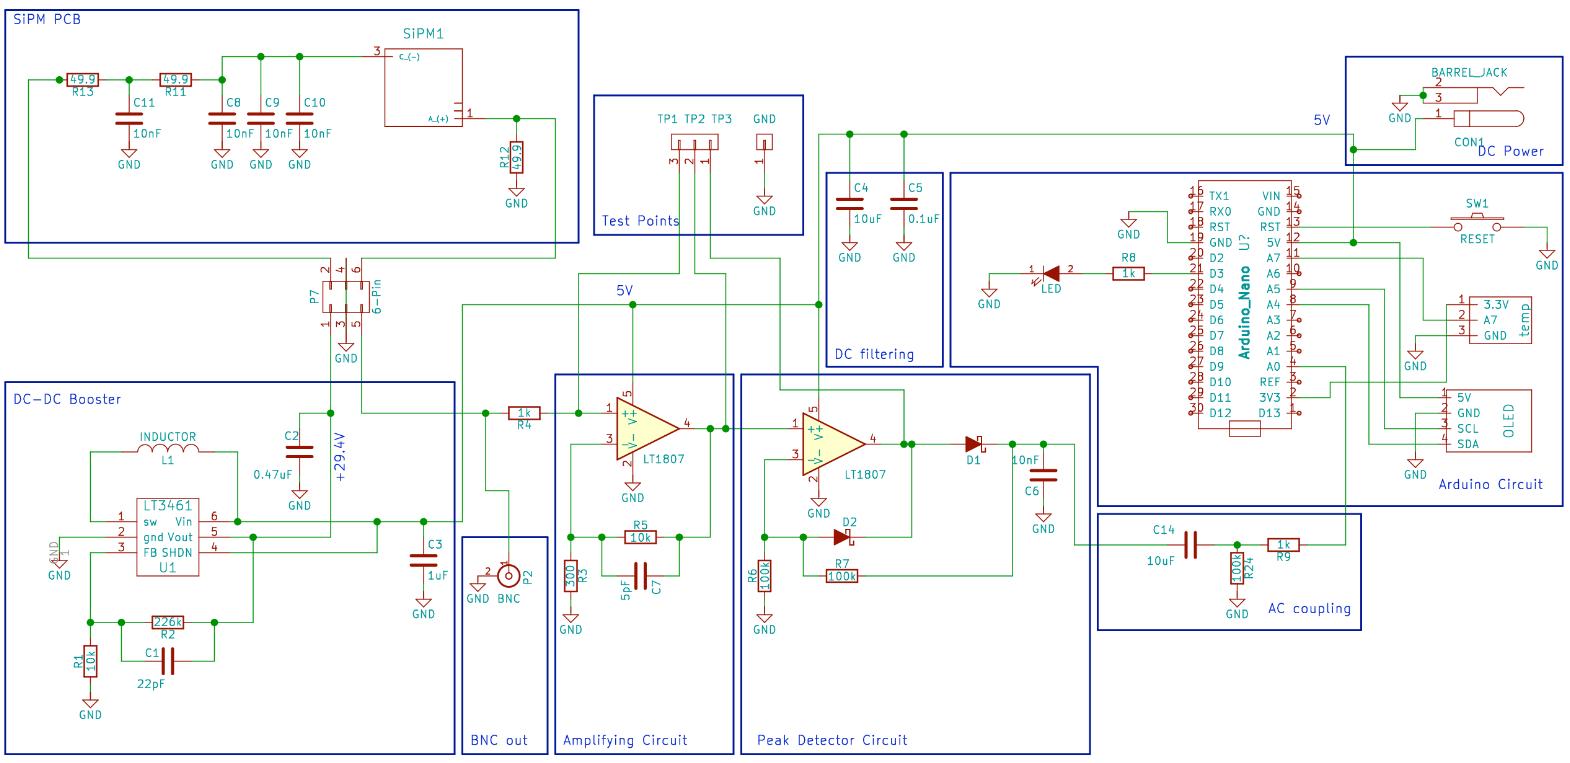
\includegraphics[width=0.8\textwidth]{Circuits.png}
    \caption{
        Schematic circuit diagram of the muon signal detecting components.
        There are SiPM, DC amplifying module, general Amplifying circuit, peak detection circuit, and DC filtering modules.
        The figure is presented by ([\cite{MuonDetection2023}])
    }
    \label{fig: total_circuit_fig}
\end{figure}

We constructed Amplifying circuit and peak detection circuit, and tested its performance in noisy nature by module 3 writeups.
They are the components of machine able to be built with op-amps.
We tested the peak noise response of such circuit simulated, and the results are successful enough that the peak counter works fine.
The rest of the modules are SiPM and scintillator, which we need to challenge for, but elecronic struggles are mostly solved.
Overall, our team is ready to dive into find muons on help of Analog Discovery 2.

\section{Financial Feasibility}
The things we need to purchase are approximately 16,000 KRW.
\begin{itemize}
    \item SiPM - 44,687 KRW -  MICROFC-60035-SMT-TR By OnSemi (ETA. 2024/11/29)
    \item Scintillator - 98,750 KRW - EJ-200 By Eljen Tech. (ETA. 2024/11/24)
    \item DC Booster - 9,223 KRW - LT3461 By EVALZ Analog Device (ETA. 2024/11/26)
    \item Delivery fee < 10,000 KRW
\end{itemize}



\section{References}
\bibliographystyle{plain} 
\bibliography{proposalref}
\end{document}